\documentclass[12pt,english]{article}
\usepackage[utf8]{inputenc}
\usepackage{geometry}
\usepackage{graphicx}
\usepackage{mathtools}
\usepackage[hidelinks]{hyperref}
\usepackage{setspace}
\usepackage{titlesec}
\usepackage{subcaption}
%\titleformat{\section}
%{\normalfont\Large\bfseries}{Exercise~\thesection}{1em}{}
\usepackage{siunitx,textcomp}
\geometry{
	a4paper,
	left=25mm,
	right=25mm,
	top=25mm,
	bottom=25mm,
}
\usepackage{babel}
\usepackage{lmodern}
\usepackage[T1]{fontenc}
\usepackage{float}
\usepackage{tikz}
\usepackage{caption}
\usepackage{pgfplots}
\pgfplotsset{compat=newest}
\usepgfplotslibrary{units}
\usepackage{standalone}
\usepackage{tikzscale}
\makeatletter
\pgfplotsset{
	unit code/.code 2 args=
	\begingroup
	\protected@edef\x{\endgroup\si{#2}}\x
}

\makeatother
\usepackage[final]{microtype}
\renewcommand{\thesection}{Exercice~\arabic{section}}

\begin{document}
	
	\begin{titlepage}
		{\setstretch{1.0}
			
			
\includegraphics[width=\textwidth]{img/Logos.pdf} \hspace{4.5cm}
			
			\vspace{1 cm}
			\large
			
			\begin{tabular}{lr}
				\begin{minipage}[t]{0.5\textwidth}
					{\small\textsc{Brussels Faculty of Enginering} \\[1ex]
						Université Libre de Bruxelles\\[1ex]
						Vrije Universiteit van Brussel\\[1ex]}
				\end{minipage} & \begin{minipage}[t]{0.45\textwidth}
					\begin{flushright}
						{\small Academic Year 2017-2018}
					\end{flushright}
				\end{minipage}
			\end{tabular}
			
			\vspace{\stretch{2}}
			\begin{center}
				\Large 
				\textbf{Labs Report}\\
				\vspace{3 cm}
				\large
				Cédric Hannotier\\ 
			\end{center}
			
			
			\vspace{\stretch{2}}
			
			\begin{minipage}[t]{\textwidth}
				\normalsize \textbf{INFO-Y093}: Image and video technology\\[1.5ex]
			\end{minipage}
		}
		
	\end{titlepage}

\tableofcontents\newpage

\section[]{\thesection}
By modifying window/level values (\autoref{fig:wlad}), we can get sharper image (\autoref{fig:wllena}) and modify its histogram. Lena histogram is shown \autoref{fig:lenah}.

\begin{figure}
	\centering
	\includegraphics[width=.8\textwidth]{tikz/windowlevel}
	\caption{Window/Level Adjustment}
	\label{fig:wlad}
\end{figure}

\begin{figure}
	\centering
	\includegraphics[width=.9\textwidth]{tikz/histogramlena}
	\caption{Histogram of Lena}
	\label{fig:lenah}
\end{figure}

\begin{figure}
	 \centering
	 \begin{subfigure}[t]{0.4\textwidth}
	 	\centering
	 	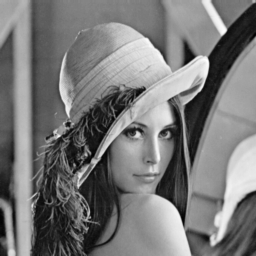
\includegraphics[width=.9\textwidth]{img/lena}
	 	\caption{Original Lena (W: 255, L: 128)}
	 	\label{fig:lenao}
	 \end{subfigure}%
	 \qquad
	 \begin{subfigure}[t]{0.4\textwidth}
	 	\centering
	 	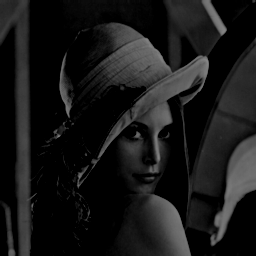
\includegraphics[width=.9\textwidth]{img/lenadark}
	 	\caption{Modified Lena (W:154, L:176)}
	 	\label{fig:lenad}
	 \end{subfigure}
	 \caption{Window/Level effects on Lena}
	 \label{fig:wllena}
\end{figure}


\section[]{\thesection}
The resulting image is shown \autoref{fig:cst} and its window/level values enclose the full range of pixel. By modifying the window/level, we can get a common checkerboard image (\autoref{fig:cstwl}). Checkerboard histogram is shown \autoref{fig:csth}.

\begin{figure}
	\centering
	\begin{subfigure}[t]{0.4\textwidth}
		\centering
		
\includegraphics[width=.9\textwidth]{img/cst}
		\caption{Original checkerboard (W: 1, L: 0.5)}
		\label{fig:cst}
	\end{subfigure}%
	\qquad
	\begin{subfigure}[t]{0.4\textwidth}
		\centering
		
\includegraphics[width=.9\textwidth]{img/cstwl}
		\caption{Modified checkerboard (W:0.01, L:0.5)}
		\label{fig:cstwl}
	\end{subfigure}
	\caption{Window/Level effects on checkerboard}
	\label{fig:checkerboard}
\end{figure}

\begin{figure}
	\centering
	\includegraphics[width=.9\textwidth]{tikz/histogramcst}
	\caption{Histogram of checkerboard}
	\label{fig:csth}
\end{figure}

\section[]{\thesection}
The mean of uniform-distributed random image in [0, 1] is 0.5 as expected. The MSE of this uniform random image compared to a 0.5 constant image is 0.0831.

A standard deviation $\sigma$ of the Gaussian-distributed random image matches the MSE of the uniform random image if $\sigma \approx 0.29$. Results are shown on \autoref{fig:uninorm}. As shown in \autoref{tab:uninorm}, standard deviations of both the images are quite similar.

\begin{figure}
	\centering
	\begin{subfigure}[t]{0.4\textwidth}
		\centering
		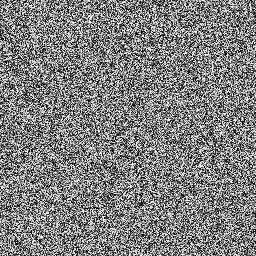
\includegraphics[width=.9\textwidth]{img/uniformImage}
		\caption{Uniform random image (W: 1, L: 0.5)}
		\label{fig:uni}
	\end{subfigure}%
	\qquad%
	\begin{subfigure}[t]{0.4\textwidth}
		\centering
		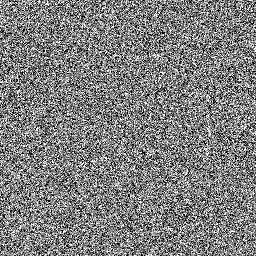
\includegraphics[width=.9\textwidth]{img/normalImage}
		\caption{Normal random image (W:1, L:0.5)}
		\label{fig:norm}
	\end{subfigure}%
	
	\begin{subfigure}[t]{0.4\textwidth}
		\centering
		\includegraphics[width=.9\textwidth]{tikz/HistogramuniformImage}
		\caption{Histogram of uniform random image}
		\label{fig:unih}
	\end{subfigure}%
	\qquad
	\begin{subfigure}[t]{0.4\textwidth}
		\centering
		\includegraphics[width=.9\textwidth]{tikz/HistogramnormalImage}
		\caption{Histogram of normal random image}
		\label{fig:normh}
	\end{subfigure}
	
	\caption{Uniform and normal random images comparison}
	\label{fig:uninorm}
\end{figure}

\begin{table}
	\centering
	\begin{tabular}{|c|c|c|c|c|}
		\hline
		& Mean & Standard deviation & Min & Max\\\hline
		Uniform & 0.5 & 0.288 & 0 & 1 \\\hline
		Normal & 0.5 & 0.29 & -0.66 & 1.89\\\hline
	\end{tabular}
	\caption{Uniform and normal random images comparison}
	\label{tab:uninorm}
\end{table}

\section[]{\thesection}
Lena images with different Gaussian noise standard deviations are shown \autoref{fig:lenag}. Noisy images have been clipped to the range [0, 1].

\begin{figure}
	\centering
	\begin{subfigure}[t]{0.4\textwidth}
		\centering
		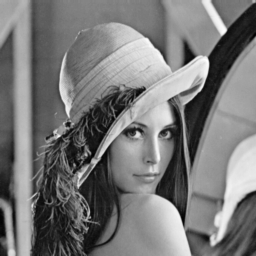
\includegraphics[width=.9\textwidth]{img/lena}
		\caption{Original Lena}
		\label{fig:orleno}
	\end{subfigure}%
	\qquad%
	\begin{subfigure}[t]{0.4\textwidth}
		\centering
		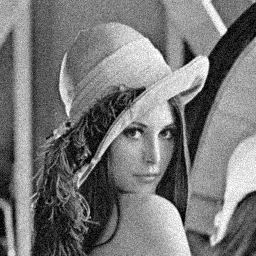
\includegraphics[width=.9\textwidth]{img/lenan1}
		\caption{$\sigma = 0.05$, $\text{PSNR}=\SI{26.07}{\decibel}$}
		\label{fig:lenag1}
	\end{subfigure}%
	
	\begin{subfigure}[t]{0.4\textwidth}
		\centering
		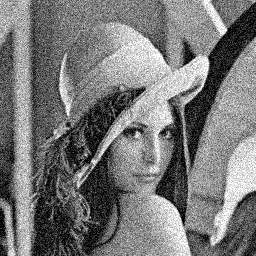
\includegraphics[width=.9\textwidth]{img/lenan2}
		\caption{$\sigma = 0.1$, $\text{PSNR}=\SI{20.24}{\decibel}$}
		\label{fig:lenag2}
	\end{subfigure}%
	\qquad
	\begin{subfigure}[t]{0.4\textwidth}
		\centering
		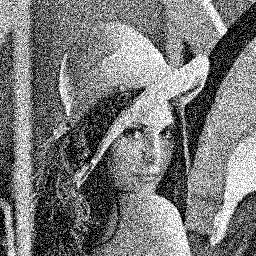
\includegraphics[width=.9\textwidth]{img/lenan3}
		\caption{$\sigma = 0.2$, $\text{PSNR}=\SI{14.69}{\decibel}$}
		\label{fig:lenag3}
	\end{subfigure}
	\caption{Gaussian noise effects}
	\label{fig:lenag}
\end{figure}

\section[]{\thesection}
The kernel can be calculated knowing the 2D Gaussian distribution (assuming $x_1, x_2$ uncorrelated, i.e. $\rho=0$, $\sigma_1=\sigma_2 = 1$):
\begin{equation}
f(x,y) = \frac{1}{2\pi}e^{-\frac{1}{2}(\sigma_1+\sigma_2)}
\end{equation}
Hence, the kernel is:
\begin{equation}
\begin{pmatrix}
f(-1,-1) & f(0,-1) & f(1,-1)\\
f(-1,0) & f(0,0) & f(1,0)\\
f(-1,1) & f(0, 1) & f(1,1)	
\end{pmatrix} \approx \begin{pmatrix}
0.0751 & 0.1238 & 0.0751\\
0.1238 & 0.2042 & 0.1238\\
0.0751 & 0.1238 & 0.0751\\
\end{pmatrix}
\end{equation}

The blurred and sharpened images are shown \autoref{fig:lenaum}. The borders are replicated to minimize border effects during the convolution. The blurred image (\autoref{fig:blur}) looks worst to my naked eyes than noisy one.

\begin{figure}
	\centering
	\begin{subfigure}[t]{0.4\textwidth}
		\centering
		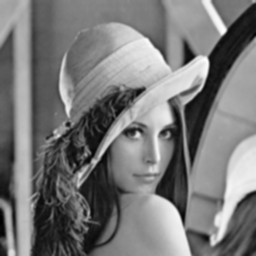
\includegraphics[width=.9\textwidth]{img/blurred}
		\caption{Blurred Lena ($\text{PSNR}=\SI{32.35}{\decibel}$)}
		\label{fig:blur}
	\end{subfigure}%
	\qquad%
	\begin{subfigure}[t]{0.4\textwidth}
		\centering
		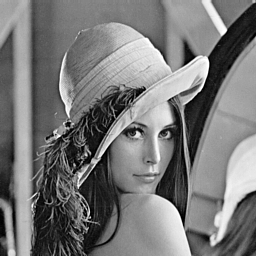
\includegraphics[width=.9\textwidth]{img/sharped}
		\caption{Sharpened Lena ($\text{PSNR}=\SI{32.48}{\decibel}$)}
		\label{fig:shap}
	\end{subfigure}
	\caption{Unshap masking on Lena}
	\label{fig:lenaum}
\end{figure}

\section[]{\thesection}
To get a similar PSNR, the standard deviation $\sigma$ of the additive Gaussian noise has been set to $0.024$.

Results are shown \autoref{fig:lenanb}. By applying blur, we average the effect of the noise by block of kernel size. Hence, it is possible to decrease the noise effect in a image by blurring it. The \autoref{fig:bnoise} models well artifacts of the SLR camera since in this kind of camera, the image is firstly blurred then, due to the electronics, noise is added.

\begin{figure}
	\centering
	\begin{subfigure}[t]{0.4\textwidth}
		\centering
		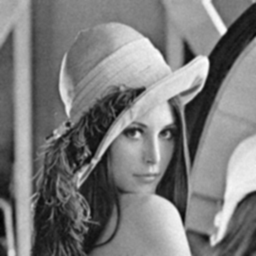
\includegraphics[width=.9\textwidth]{img/nblur}
		\caption{Noise + blur Lena ($\text{PSNR}=\SI{31.84}{\decibel}$)}
		\label{fig:nblur}
	\end{subfigure}%
	\qquad%
	\begin{subfigure}[t]{0.4\textwidth}
		\centering
		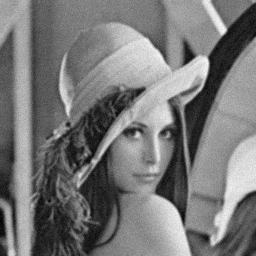
\includegraphics[width=.9\textwidth]{img/bnoise}
		\caption{Blur + noise Lena ($\text{PSNR}=\SI{29.34}{\decibel}$)}
		\label{fig:bnoise}
	\end{subfigure}
	\caption{Blurring and noise effects on Lena}
	\label{fig:lenanb}
\end{figure}
\setcounter{section}{7}

\section[]{\thesection}
DCT and IDCT bases dictionaries are shown \autoref{fig:iddct}. The one is the transposed of the other (difficult to see). The DC coefficient, after rescaling, is equal to $\frac{1}{\sqrt{2}}\approx 0.707$.

By thresholding, we are losing information, hence the quality of the image decreases. Results for different thresholds are shown \autoref{fig:tlena}.

\begin{figure}
	\centering
	\begin{subfigure}[t]{0.4\textwidth}
		\centering
		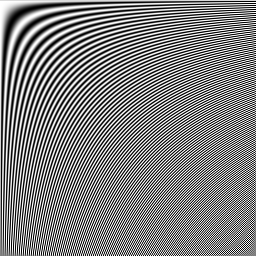
\includegraphics[width=.9\textwidth]{img/DCT_vectors}
		\caption{DCT basis}
		\label{fig:dct}
	\end{subfigure}%
	\qquad%
	\begin{subfigure}[t]{0.4\textwidth}
		\centering
		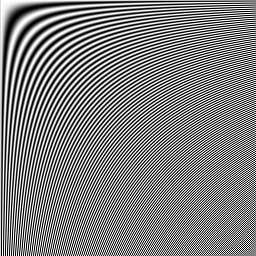
\includegraphics[width=.9\textwidth]{img/IDCT_vectors}
		\caption{IDCT basis}
		\label{fig:idct}
	\end{subfigure}
	\caption{(I)DCT bases}
	\label{fig:iddct}
\end{figure}

\begin{figure}
	\centering
	\begin{subfigure}[t]{0.3\textwidth}
		\centering
		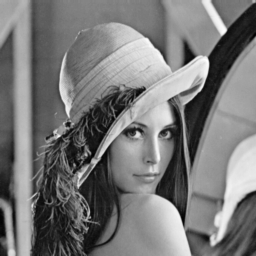
\includegraphics[width=.9\textwidth]{img/lena}
		\caption{DCT basis}
		\label{fig:lenaoo}
	\end{subfigure}%
	\quad%
	\begin{subfigure}[t]{0.3\textwidth}
		\centering
		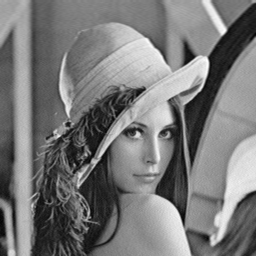
\includegraphics[width=.9\textwidth]{img/lena_new_t10}
		\caption{Threshold of 10, $\text{PSNR}=\SI{37.43}{\decibel}$}
		\label{fig:lzna10}
	\end{subfigure}
	\quad%
	\begin{subfigure}[t]{0.3\textwidth}
		\centering
		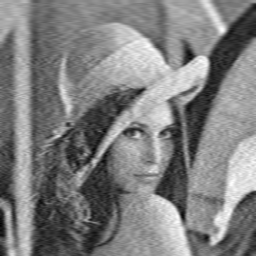
\includegraphics[width=.9\textwidth]{img/lena_new_t50}
		\caption{Threshold of 50, $\text{PSNR}=\SI{25.26}{\decibel}$}
		\label{fig:lena50}
	\end{subfigure}
	\caption{Thresholding effects on Lena}
	\label{fig:tlena}
\end{figure}

\section[]{\thesection}
The $Q$ matrix is shown \autoref{fig:Q}. Knowing the lighter is the color, higher is the value. That means high frequencies coefficients need higher absolute values to be as significant as lower frequencies coefficients.

The Q matrix coefficients were certainly set empirically, it is asymmetric because better quality was observed than symmetric one.

Analysis of JPEG quality is shown \autoref{fig:jqlena}. Even if it is difficult to see visual differences in \autoref{fig:jlena} and \ref{fig:j50lena}, quantitatively differences are non negligible (\autoref{fig:dlena}). Most of differences are present at edges in the image (edges $\to$ high frequencies).

\begin{figure}
	\centering
	
\includegraphics[width=.4\textwidth]{img/Q}
	\caption{$\SI{50}{\percent}\, Q$ matrix}
	\label{fig:Q}
\end{figure}

\begin{figure}
	\centering
	\begin{subfigure}[t]{0.3\textwidth}
		\centering
		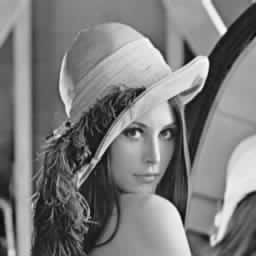
\includegraphics[width=.9\textwidth]{img/lenaJPEG}
		\caption{JPEG version of Lena}
		\label{fig:jlena}
	\end{subfigure}%
	\quad%
	\begin{subfigure}[t]{0.3\textwidth}
		\centering
		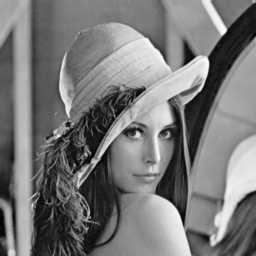
\includegraphics[width=.9\textwidth]{img/lenaJPEG8bpp}
		\caption{JPEG version of Lena ($Q=\SI{50}{\percent}$, $\text{PSNR}=\SI{32.61}{\decibel}$)}
		\label{fig:j50lena}
	\end{subfigure}
	\quad%
	\begin{subfigure}[t]{0.3\textwidth}
		\centering
		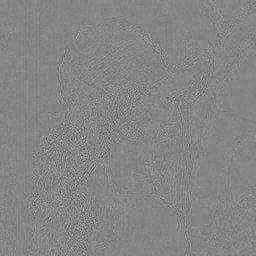
\includegraphics[width=.9\textwidth]{img/ResultoflenaJPEG}
		\caption{Difference due to loss}
		\label{fig:dlena}
	\end{subfigure}
	\caption{Lossy JPEG}
	\label{fig:jqlena}
\end{figure}

\section[]{\thesection}
Both packings are shown \autoref{fig:cidctc}. The interleaved version regroups the coefficients by frequency. This representation is similar to DWT decomposition (with sub-level). That representation can be use for scalability when reconstructing.
 
\begin{figure}
	\centering
	\begin{subfigure}[t]{0.4\textwidth}
		\centering
		
\includegraphics[width=.9\textwidth]{img/lenaJPEG8}
		\caption{Contiguous DCT coefficients}
		\label{fig:cdctc}
	\end{subfigure}%
	\qquad%
	\begin{subfigure}[t]{0.4\textwidth}
		\centering
		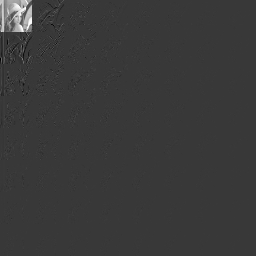
\includegraphics[width=.9\textwidth]{img/lenaJPEG32}
		\caption{Interleaved DCT coefficients}
		\label{fig:idctc}
	\end{subfigure}
	\caption{DCT packing}
	\label{fig:cidctc}
\end{figure}


\section[]{\thesection}
\textit{C.f.} \autoref{ici}
\section[]{\thesection}
\textit{C.f.} \autoref{ici}
\section[]{\thesection}\label{ici}
The probability density function (non normalized) are represented \autoref{fig:test}. The longer run is 375 and there is 5375 runs. After normalize the pdf, the entropy can be calculated using \eqref{eq:blblb} and is equal to \SI{4.59}{bits/run}. Hence, an ideal entropy encoder will compress the runs in \SI{24681.09}{bits}.

After the creation of a LUT to link most probable runs with shortest golomb code, the compressed file contains \SI{27371}{bits} (without the LUT).
\begin{equation}\label{eq:blblb}
H = -p_i\sum_i^N p_i\log_2p_i
\end{equation}
\begin{figure}
	\centering
	\includegraphics[width=.9\textwidth]{tikz/test}
	\caption{runs pdf}
	\label{fig:test}
\end{figure}

	
\end{document}